\chapter{Resultados} \label{resultados}

Nesse capítulo são detalhados os resultados obtidos em cada faze do processo de
KDD aplicado nesse trabalho. Ele está nas mesmas seções do capítulo anterior,
pois cada faze do KDD contribui para o resultado final do processo e gera seus
próprios artefatos.

\section{Entrada de dados}

Para a etapa de entrada de dados, foram desenvolvidos \textit{scripts} em SQL
que criavam tabelas na base de dados em MySQL com subconjuntos de dados
relacionados com os cursos selecionados para esse estudo. Esses \textit{scripts}
estão disponíveis no Anexo \ref{anex:anexo1}. O Quadro \ref{reducedDataTables}
apresenta e resume essas tabelas auxiliares.

\begin{quadro}[!htb]
  \centering
  \caption{Descrição das tabelas criadas apenas com dados dos cursos selecionados}
  \label{reducedDataTables}
  \begin{tabular}{|l|l|}
    \hline
    \multicolumn{1}{|c|}{\textbf{Tabela}} & \multicolumn{1}{c|}{\textbf{Descrição}} \\ \hline
    \textit{adm} & \begin{tabular}[c]{@{}l@{}}Tabela base agrupando dados de cada aluno do curso \\ Bacharelado em Administração Pública em cada \\ disciplina em que ele cursou.\end{tabular} \\ \hline
    \textit{adm\_base\_log\_reduzido} & \begin{tabular}[c]{@{}l@{}}Tabela com registros de log dos alunos e cursos do curso\\ Bacharelado em Administração Pública.\end{tabular} \\ \hline
    \textit{adm\_disciplinas} & \begin{tabular}[c]{@{}l@{}}Registra o identificador das disciplinas do curso de\\ Bacharelado em Administração Pública, data de início \\ e data de fim.\end{tabular} \\ \hline
    \textit{adm\_id\_alunos} & \begin{tabular}[c]{@{}l@{}}Registra o identificador dos alunos matriculados no \\ curso de Bacharelado em Administração Pública.\end{tabular} \\ \hline
    \textit{lic\_ped} & \begin{tabular}[c]{@{}l@{}}Tabela base agrupando dados de cada aluno do curso \\ Licenciatura em Pedagogia em cada disciplina\\ em que ele cursou.\end{tabular} \\ \hline
    \textit{lic\_ped\_base\_log\_reduzido} & \begin{tabular}[c]{@{}l@{}}Tabela com registros de log dos alunos e cursos do curso\\ Licenciatura em Pedagogia.\end{tabular} \\ \hline
    \textit{lic\_ped\_disciplinas} & \begin{tabular}[c]{@{}l@{}}Registra o identificador das disciplinas do curso de\\ Licenciatura  em Pedagogia, data de início e data de fim.\end{tabular} \\ \hline
    \textit{lic\_ped\_id\_alunos} & \begin{tabular}[c]{@{}l@{}}Registra o identificador dos alunos matriculados no\\  curso de Licenciatura em Pedagogia.\end{tabular} \\ \hline
  \end{tabular}
  \Ididthis
\end{quadro}

Essas tabelas se tornaram necessárias, pois, executar \textit{scripts} que
buscassem dados em toda a base do Moodle demandava horas de processamento. Em
contrapartida, utilizando apenas essas tabelas o tempo de execução foi reduzido
para poucos minutos.

\section{Pré-processamento}

Utilizando as tabelas do Quadro \ref{reducedDataTables} e os \textit{scripts}
disponíveis no Anexo \ref{anex:anexo1}, as variáveis, mapeadas para construtos
da TDT por \citeonline{ramos2016abordagem}, foram salvas como valores em uma
tabela cujas colunas eram os identificadores listados no Quadro
\ref{variablesDescritionTable}.

\begin{quadro}[!htb]
  \centering
  \caption{Lista das variáveis e respectivos construtos e seus identificadores}
  \label{variablesDescritionTable}
  \begin{tabular}{|l|l|l|}
    \hline
    \multicolumn{1}{|c|}{\textbf{Identificador}} & \multicolumn{1}{c|}{\textbf{Variáveis}} & \multicolumn{1}{c|}{\textbf{Construto}} \\ \hline
    VAR01 & \begin{tabular}[c]{@{}l@{}}Quantidade geral de postagens do aluno em fóruns,\\ por disciplina.\end{tabular} & Diálogo \\ \hline
    VAR02 & \begin{tabular}[c]{@{}l@{}}Quantidade geral de mensagens enviadas pelo\\ aluno dentro do ambiente, por semestre.\end{tabular} & Diálogo \\ \hline
    VAR03 & \begin{tabular}[c]{@{}l@{}}Quantidade geral de mensagens recebidas pelo\\ aluno dentro do ambiente, por semestre.\end{tabular} & Diálogo \\ \hline
    VAR04 & \begin{tabular}[c]{@{}l@{}}Quantidade geral de recursos disponibilizados pelo\\ professor (página web, vídeo, pdfs, entre outros)\\ por disciplina.\end{tabular} & Estrutura \\ \hline
    VAR05a & \begin{tabular}[c]{@{}l@{}}Quantidade de acessos do aluno ao ambiente por\\ turno (Manhã), por semestre.\end{tabular} & Autonomia \\ \hline
    VAR05b & \begin{tabular}[c]{@{}l@{}}Quantidade de acessos do aluno ao ambiente por\\ turno (Tarde), por semestre.\end{tabular} & Autonomia \\ \hline
    VAR05c & \begin{tabular}[c]{@{}l@{}}Quantidade de acessos do aluno ao ambiente por\\ turno (Noite), por semestre.\end{tabular} & Autonomia \\ \hline
    VAR06 & \begin{tabular}[c]{@{}l@{}}Quantidade de colegas diferentes para quem o\\ aluno enviou mensagens no ambiente, por\\ semestre.\end{tabular} & Diálogo \\ \hline
    VAR07 & \begin{tabular}[c]{@{}l@{}}Quantidade de acessos do aluno ao ambiente no\\ semestre.\end{tabular} & Autonomia \\ \hline
    VAR08 & \begin{tabular}[c]{@{}l@{}}Quantidade de mensagens enviadas pelo aluno\\ aos professores pelo ambiente, por semestre.\end{tabular} & Diálogo \\ \hline
    VAR09 & \begin{tabular}[c]{@{}l@{}}Quantidade de mensagens dos professores recebidas\\ pelo aluno no ambiente, por semestre.\end{tabular} & Diálogo \\ \hline
    VAR10 & \begin{tabular}[c]{@{}l@{}}Quantidade de mensagens de colegas recebidas pelo\\ aluno no ambiente, por semestre.\end{tabular} & Diálogo \\ \hline
    VAR11 & \begin{tabular}[c]{@{}l@{}}Quantidade de mensagens enviadas pelo aluno para\\ outros colegas no ambiente, por semestre.\end{tabular} & Diálogo \\ \hline
    VAR12 & \begin{tabular}[c]{@{}l@{}}Quantidade de atividades com prazos de resposta ou\\ envio definidos por professor, por disciplina.\end{tabular} & Estrutura \\ \hline
    VAR13 & \begin{tabular}[c]{@{}l@{}}Quantidade de acessos do aluno aos diferentes tipos\\ de atividades disponibilizadas (webquest, fórum,\\ quiz, entre outros), por disciplina.\end{tabular} & Autonomia \\ \hline
    VAR14 & \begin{tabular}[c]{@{}l@{}}Quantidade de fóruns de discussão disponibilizados\\ sobre os conteúdos por disciplina.\end{tabular} & Estrutura \\ \hline
    VAR15 & \begin{tabular}[c]{@{}l@{}}Quantidade de acessos do aluno aos fóruns, por\\ disciplina.\end{tabular} & Autonomia \\ \hline
  \end{tabular}
  \Otherguydidthis{ramos2016abordagem}
\end{quadro}

Além das variáveis, cada linha possui o identificador de um aluno e de uma
disciplina. Dessa forma, cada linha representa um aluno em uma disciplina do
curso.

Essas tabelas foram coneconvertidasrtidas para planilhas eletrônicas para facilitar o
processo de correção e validação dos resultados. As planilhas serviram como base
para os processos de mineração de dados.

\section{Mineração de Dados}

As planilhas eletrônicas foram carregadas em \textit{dataframes}, como foi
descrito no capítulo \ref{metodos}.

Os dados do curso de Licenciatura em Pedagogia somaram 6240 entradas. Sendo que,
$50,6\%$ foram marcados como não evadidos e $49,4\%$ foram marcados como
evadido, como ilustra a Figura \ref{classDistribuitionPedTotal}. A proporção das
classes após a divisão dos dados em conjunto de testes e conjunto de treinamento
é mostrada nas Figuras \ref{classDistribuitionPedTest} e
\ref{classDistribuitionPedTrain}, respectivamente.

\begin{figure}[!htb]
  \centering
  \caption{\label{classDistribuitionPed} Distribuição de classes para os dados do curso de Licenciatura em Pedagogia.}
  \subcaptionbox{\label{classDistribuitionPedTotal}Distribuição em todos os dados.}{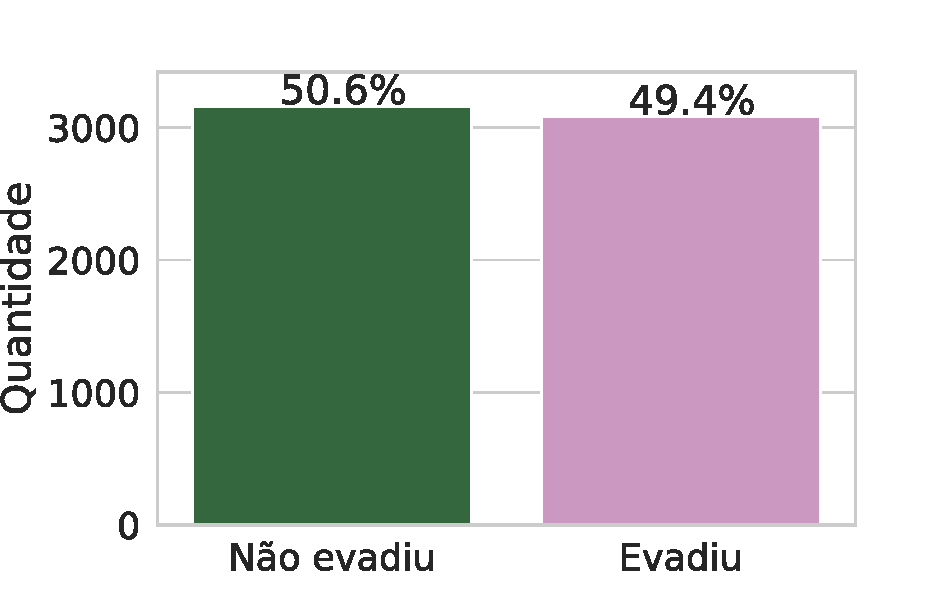
\includegraphics[scale=.47]{img/barplot_pedagogia}}\qquad
  \subcaptionbox{\label{classDistribuitionPedTest}Distribuição para os dados de teste.}{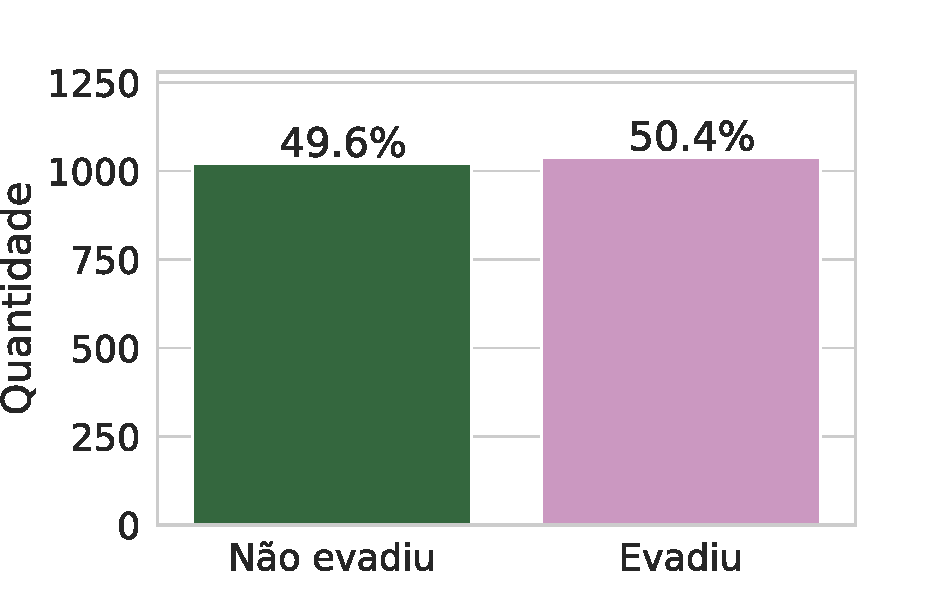
\includegraphics[scale=.47]{img/barplot_pedagogia_testes}}\qquad
  \subcaptionbox{\label{classDistribuitionPedTrain}Distribuição para os dados de treinamento.}{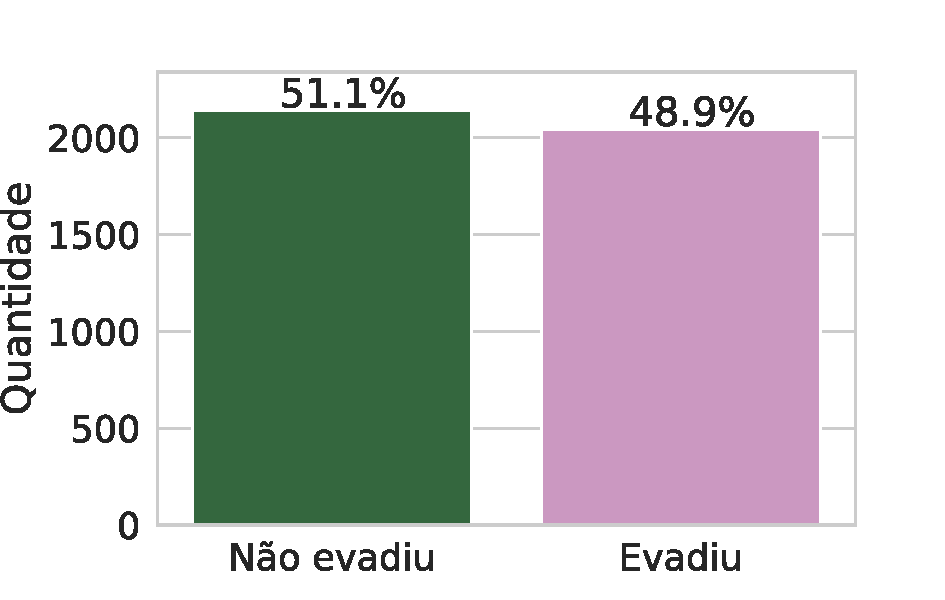
\includegraphics[scale=.47]{img/barplot_pedagogia_treinamento}}
  \vspace{1.5em}
  \Ididthis
\end{figure}

Os dados do curso de Bacharelado em Administração Pública somaram 11689
entradas. Sendo que, $43,9\%$ foram marcados como não evadidos e $56,1\%$ foram
marcados como evadido, como ilustra a Figura \ref{classDistribuitionAdmTotal}. A
proporção das classes após a divisão dos dados em conjunto de testes e conjunto
de treinamento é mostrada nas Figuras \ref{classDistribuitionAdmTest} e
\ref{classDistribuitionAdmTrain}, respectivamente.

\begin{figure}[!htb]
  \centering
  \caption{\label{classDistribuitionAdm} Distribuição de classes para os dados do curso de Bacharelado em Administração Pública.}
  \subcaptionbox{\label{classDistribuitionAdmTotal}Distribuição em todos os dados.}{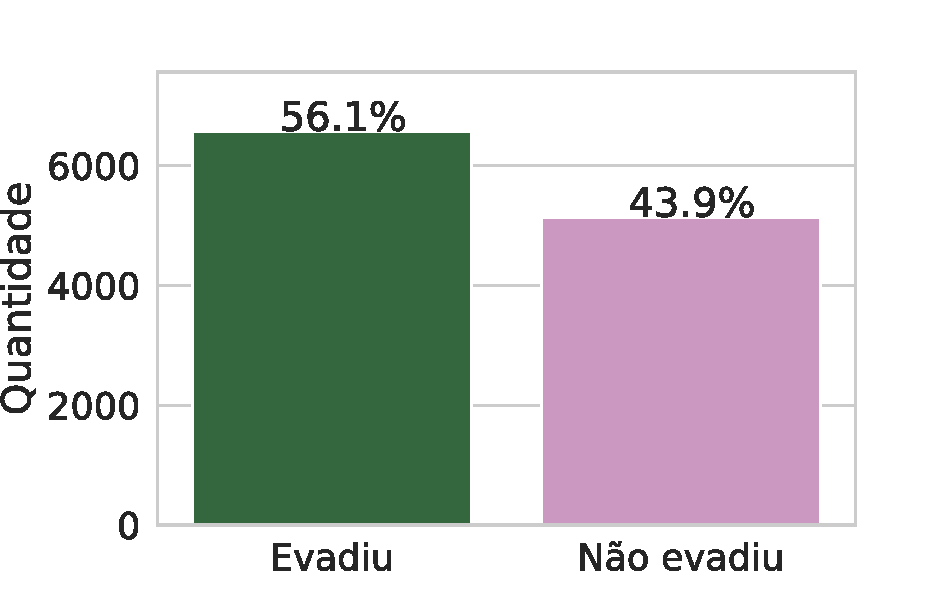
\includegraphics[scale=.47]{img/barplot_adm}}\qquad
  \subcaptionbox{\label{classDistribuitionAdmTest}Distribuição para os dados de teste.}{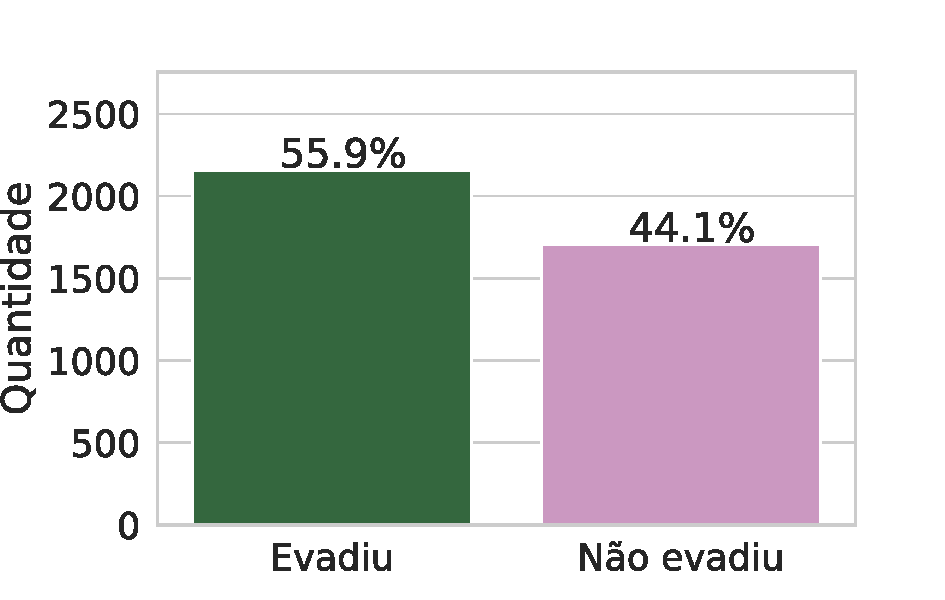
\includegraphics[scale=.47]{img/barplot_adm_testes}}\qquad
  \subcaptionbox{\label{classDistribuitionAdmTrain}Distribuição para os dados de treinamento.}{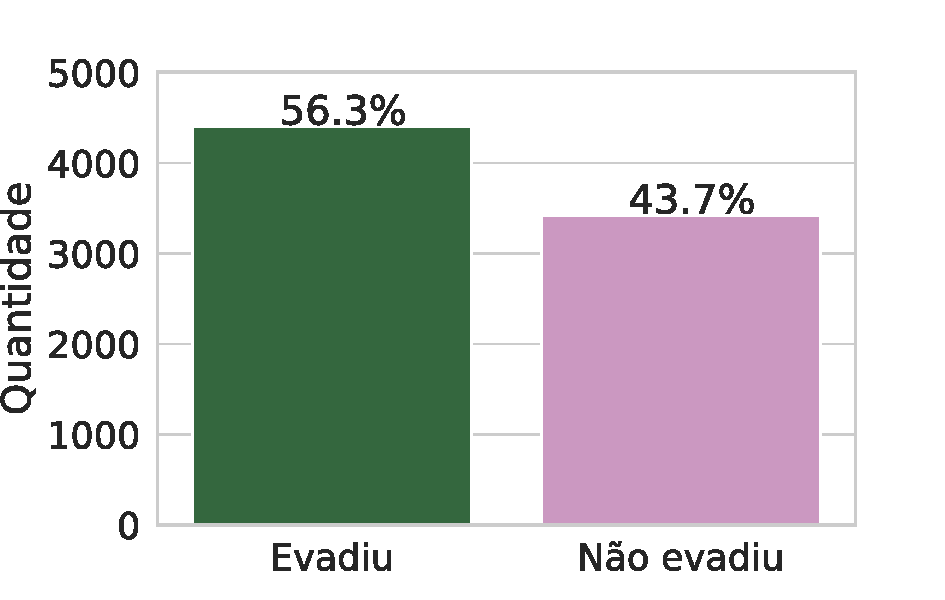
\includegraphics[scale=.47]{img/barplot_adm_treinamento}}
  \vspace{1.5em}
  \Ididthis
\end{figure}

As Tabelas \ref{decribingStatisticsPed} e \ref{decribingStatisticsPed}
apresentam as estatísticas descritivas das variáveis coletadas no curso de
Licenciatura em Pedagogia e Bacharelado em Administração Pública,
respectivamente.

\section{Pós-processamento}

\section{Conhecimento Obtido}
